\chapter{Related Work}
\label{cha:chapter3}


This chapter gives a look at the main ideas in blockchain scalability and introduces the core project on which this thesis is based.

\section{Scalability Approaches}
Various strategies are being explored to enhance blockchain scalability. Some are already operational, while others are in the research stage. These strategies broadly fall into two categories: Layer 1 and Layer 2 solutions \cite{tyagi_study_2021,thibault_blockchain_2022}. Layer 1 solutions focus on boosting blockchain scalability through means like enlarging block sizes or implementing Sharding. In contrast, Layer 2 solutions attempt to scale the blockchain by relocating computation off-chain. Noteworthy examples of Layer 2 solutions are State Channels, Sidechains, and Rollups, as illustrated in Figure \ref{fig:3_scalingSolutions}.

The common path for making blockchains handle more transactions is to use Layer 2 solutions. Many members of the Ethereum community are following this approach \cite{neiheiser_practical_2023}.

\begin{figure}[ht]
  \centering
  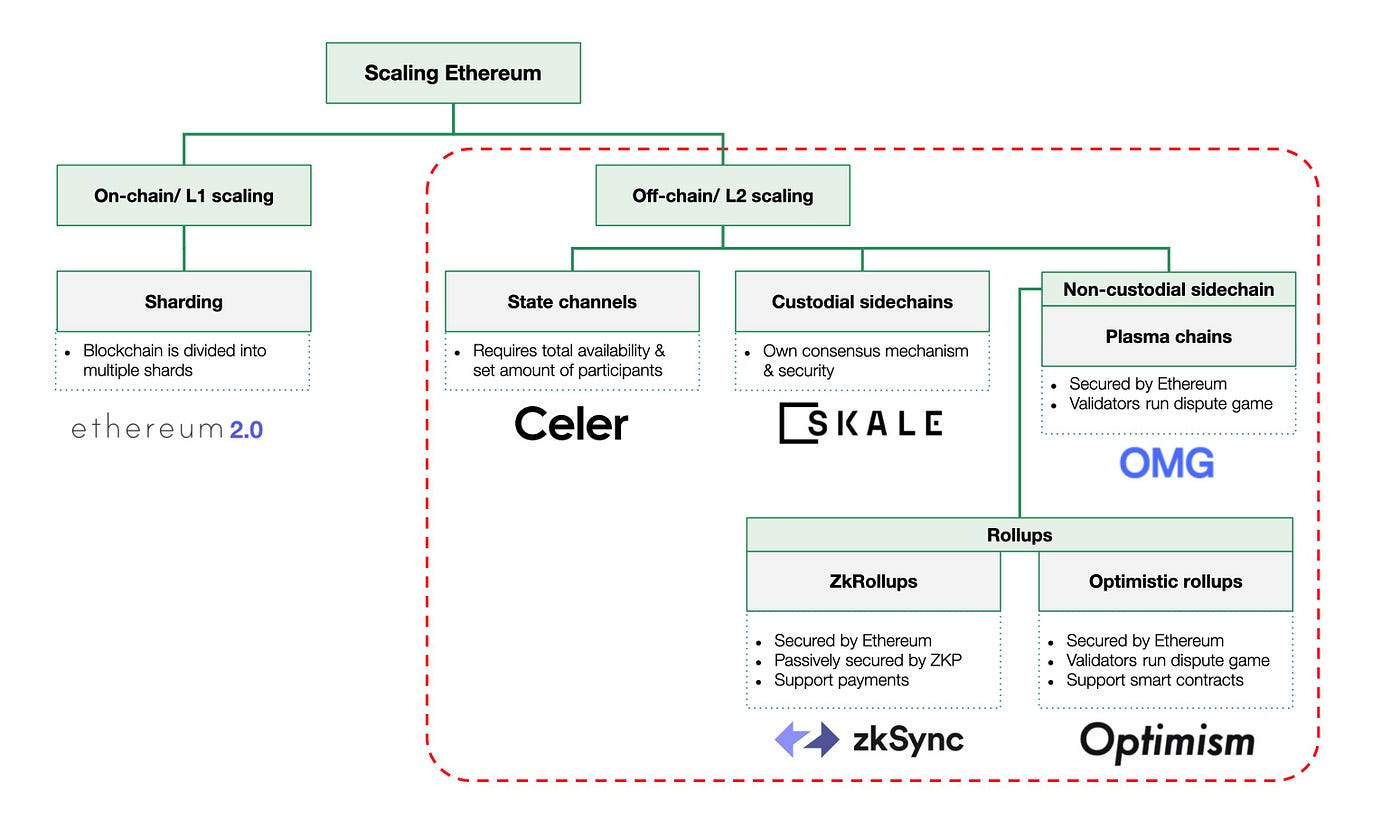
\includegraphics[width=0.95\columnwidth]{2_scalingSolutions.jpg}
  \caption[Scaling Solutions]{Principal scaling solutions for Layer 1 and Layer 2\footnotemark}  
  \label{fig:3_scalingSolutions}
\end{figure} 
\footnotetext{\url{https://medium.com/token-terminal/a-primer-on-ethereum-l2-scaling-techniques-17ac437891b1}}

\section{Zk-Rollups}
\label{sec:2_zkRollups}
Zero-Knowledge Rollups represent a Layer 2 scaling approach that takes advantage of capabilities of zero-knowledge proofs to facilitate off-chain computation. This strategy aims to alleviate the scalability limitations of blockchains by shifting most of the computational work away from the main chain while still maintaining the security and trustless nature of the system. In the context of Zk-Rollups, computation is executed off-chain, and the outcomes of these computations, accompanied by a proof of verifiably correct execution, are transmitted to the corresponding smart contract on the blockchain \cite{tyagi_study_2021}.

Figure \ref{fig:3_zkRollup_schema} illustrates the fundamental steps of the Zk-Rollup, explained by this sequence list:
\begin{enumerate}
  \item \textbf{Transaction Initiation:} Users initiate transactions with an off-chain processing node. This node is responsible for collecting and batching multiple transactions together;
  \item \textbf{Off-chain Computation:} The processing node performs computations off-chain, fetching the current state from the underlying blockchain;
  \item \textbf{Proof Transmission:} After processing the transaction batch, the node generates a proof attesting to the validity of the computations performed. This proof, along with the resulting transaction outcomes, is then transmitted to the blockchain's smart contract;
  \item \textbf{Proof Verification:} The smart contract receives the proof and checks its correctness. This step involves cryptographic operations to confirm that the computation was executed correctly and honestly;
  \item \textbf{State Update:} If the proof verification is successful, the smart contract updates its internal state on the blockchain to store the outcomes of the off-chain computation. This ensures that the blockchain remains in sync with the results of the computations performed in the Layer 2 solution.
\end{enumerate}

\begin{figure}[ht]
  \centering
  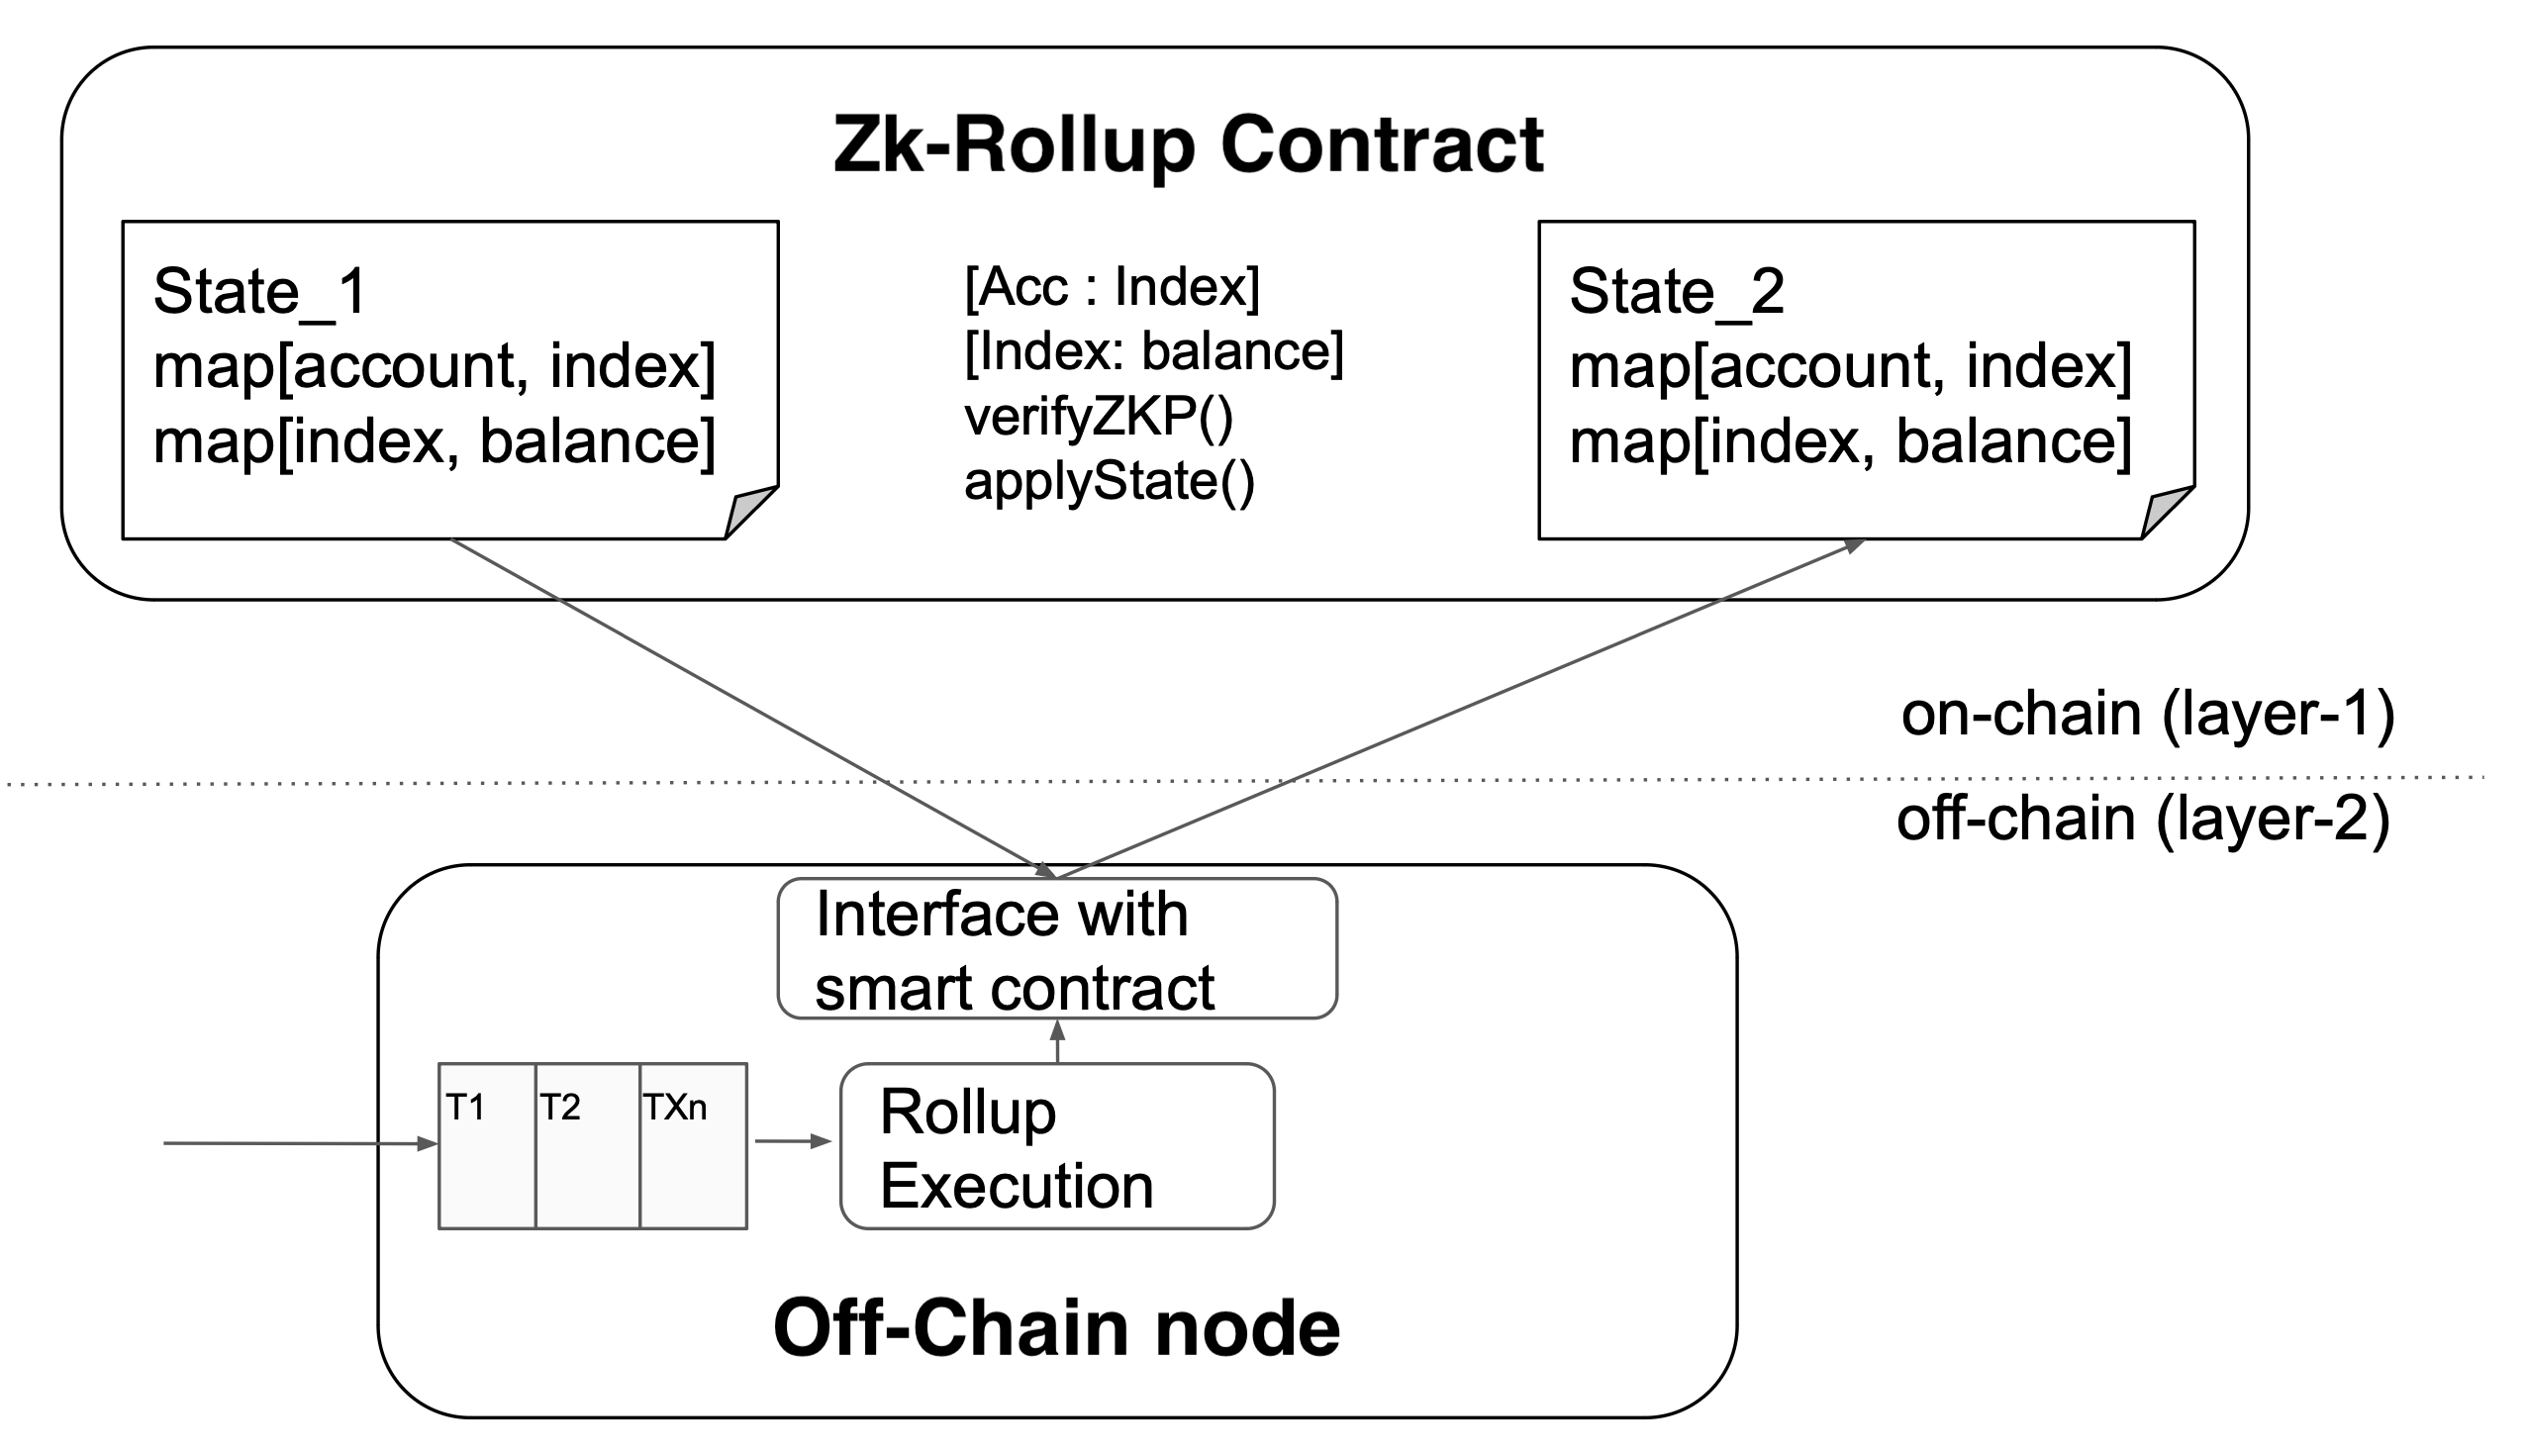
\includegraphics[width=0.95\columnwidth]{2_zkRollup_architecture.png}
  \caption[Zk-Rollup Schema]{General schema of a Zk-Rollup\cite{ise_department_tub_material_nodate}}  
  \label{fig:3_zkRollup_schema}
\end{figure}

\subsection{Zk-Rollup Implementations}
Some other Zk-Rollup implementations exist, particularly for Ethereum. The implementation discussed in \cite{dinh_implementation_2023} shares similarities with the ADSP project's approach. However, it lacks considerations for system scaling and handling multiple token types. Another example is Polygon Zero\footnote{\url{https://polygon.technology/blog/introducing-plonky2}}, which facilitates parallel execution of transactions on L2. This system blends STARK and SNARK, differing from the approach outlined in this thesis. \cite{rybakken_intmax2_2023} presents an innovative approach to Zk-Rollup featuring stateless and decentralized block production, trying to limit the data stored on chain and moving the computations to the client-side. However, this approach follows a different path from the one presented in this thesis, which uses a more classic approach with a centralized smart contract and a decentralized node.

\subsection{Zk-Rollup Reviews}
Some studies have assessed the viability and performance of the Zk-Rollup system. \cite{capko_state_2022} offers an overview of prevalent zero-knowledge proofs. The ZoKrates Toolbox, utilized by the ADSP project, employs SNARK, which requires a trusted setup phase—a potential drawback compared to Transparent zk-SNARK \cite{zhou_overview_2022}. \cite{neiheiser_practical_2023} highlights the scalability bottleneck L2 solutions may face due to a possible slow L1, constraining them below theoretical L2 throughput. \cite{starkware_fractal_2021} proposes a new Layer 3 to overcome this issue.

\section{Alternative L2 Solutions}
Several Layer 2 strategies exist to scale blockchains, offering different approaches to address the scalability challenges faced by the blockchain. Below is a brief overview at some of these strategies.

\subsection{Plasma}
Plasma presents a dynamic off-chain transaction processing solution by introducing child chains or sidechains linked to the main blockchain. These connected chains, or Plasma chains, allow for a significant increase in transaction throughput by handling transactions off the main chain. This results in faster and more efficient transactions. However, Plasma's architecture introduces a challenge: the need for resolving disputes that may arise due to potentially fraudulent or incorrect actions on these child chains\cite{thibault_blockchain_2022}. This dispute resolution process is necessary to maintain the security and integrity of the system. An example of a project utilizing the Plasma approach is OMG Network\footnote{\url{https://docs.omg.network}}, which uses Plasma chains to enhance transaction scalability while relying on the security guarantees of the main Ethereum blockchain.

\subsection{State Channels}
State channels provide a different Layer 2 scaling solution that focuses on specific use cases such as micropayments and gaming interactions. These channels allow users to execute transactions directly with each other off the main blockchain, thus reducing the congestion on the main chain and enabling faster, low-cost transactions\cite{negka_blockchain_2021}. State channels work by locking a certain amount of cryptocurrency on the blockchain and then allowing multiple off-chain transactions to occur between participants. These transactions are only confirmed on the main chain when the participants want to close the channel or when a dispute arises. An example of a project implementing state channels is Perun\footnote{\url{https://perun.network/wp-content/uploads/Perun2.0.pdf}}, which offers a framework for efficient state channel networks.

\subsection{Optimistic Rollups \label{subsec:optimisticRollups}}
Optimistic Rollups offer a compromise between transaction speed and security by assuming the validity of transactions by default\cite{thibault_blockchain_2022}. In this approach, transactions are processed quickly on Layer 2, but the verification of these transactions is postponed to the main blockchain only if disputes arise. This optimistic assumption speeds up the entire transaction processing while maintaining the chance for arbitration if necessary. It's worth noting that the vast majority of transactions are expected to be valid, so this approach optimizes for the common case. Optimistic Rollups combine the efficiency benefits of Layer 2 scaling with the security guarantees of the main blockchain. A notable downside of this solution is the presence of a long waiting time for a transaction to be confirmed on the main chain. This is due to the need of waiting for the maximum possible duration during which a dispute could potentially be raised within a rollup execution, which is called the challenge period \cite{negka_blockchain_2021}. This challenge period can last for about one week before a transaction is confirmed on the main chain.


